% !TEX root = MainDoc.tex

\usepackage[utf8]{inputenc}
\usepackage[american]{babel}
\usepackage[left=2.5cm,right=5.5cm,top=4.5cm,bottom=2.4cm]{geometry}
%\usepackage[T1]{fontenc}

\usepackage{amsmath}
\usepackage{amsfonts}
\usepackage{amssymb}
\usepackage{graphicx}
\usepackage{subfig} %supports subfigures
\usepackage{pgfplots}
\usepackage{tikz}
%Change: no more fancy in future!
\usepackage{fancyhdr}
\usepackage{multirow} % supports multiple table rows
\usepackage{colortbl} % color your tables
\usepackage{color} 
\usepackage{transparent} 
\usepackage{floatflt} %wrap text around pics 
\usepackage{float} %wrap text around pics
\usepackage{wrapfig} %wrap text around pics
\usepackage{epstopdf} %eps to pdf 
\usepackage{pdflscape} 
\usepackage{tabularx} 
\usepackage{xcolor} 
\usepackage{setspace} %line space
\usepackage{acronym} %List of abbreviations. To print only used abbr. add parameter: [printonlyused]
\usepackage[per=slash,
            decimalsymbol=comma,
            loctolang={DE:ngerman,UK:english},
            ]{siunitx} 
\usepackage{nicefrac} %nice fraq
\usepackage{rotating}
\usepackage{ragged2e}
\usepackage{pdfpages} 

%%%Settings

\pgfkeys{/pgf/number format/.cd ,use comma ,set thousands separator={.}} % thousands separator ="." instead of ","
\pgfplotsset{ every axis label/.append style={font=\scriptsize}, % 
every tick label/.append style={font=\scriptsize}} % global setting

%print only one bar in bar chart
\pgfplotsset{/pgfplots/ybar legend/.style={
		/pgfplots/legend image code/.code={\draw[##1,/tikz/.cd,bar
width=3pt,yshift=-0.2em,bar shift=0pt] plot coordinates {(0cm,0.8em)

};},
	}}

\pgfplotsset{compat=newest}
\usepgfplotslibrary{units}

\sisetup{exponent-product = \cdot, output-product = \cdot} %dot insead of "x" for scientific annotation using siunitx
%Style for list of formulas
\newcommand{\acrounit}[1]{
  \acroextra{\makebox[18mm][l]{\si{#1}}}
}


\setcounter{secnumdepth}{4} %depth chapter numbering
\setlength{\parindent}{0pt} %indent new paragraph
%Change: no more fancy in future!
\pagestyle{fancy}


%%%Header and footer settings
%Space to header
\renewcommand{\chapterheadstartvskip}{\vspace{0cm}}
%Will be changed: no more fancy in future!
\fancypagestyle{plain} %print header and footer on all sites, chapter beginnings included

\fancyhead[L]{}
\fancyhead[C]{}
\fancyhead[R]{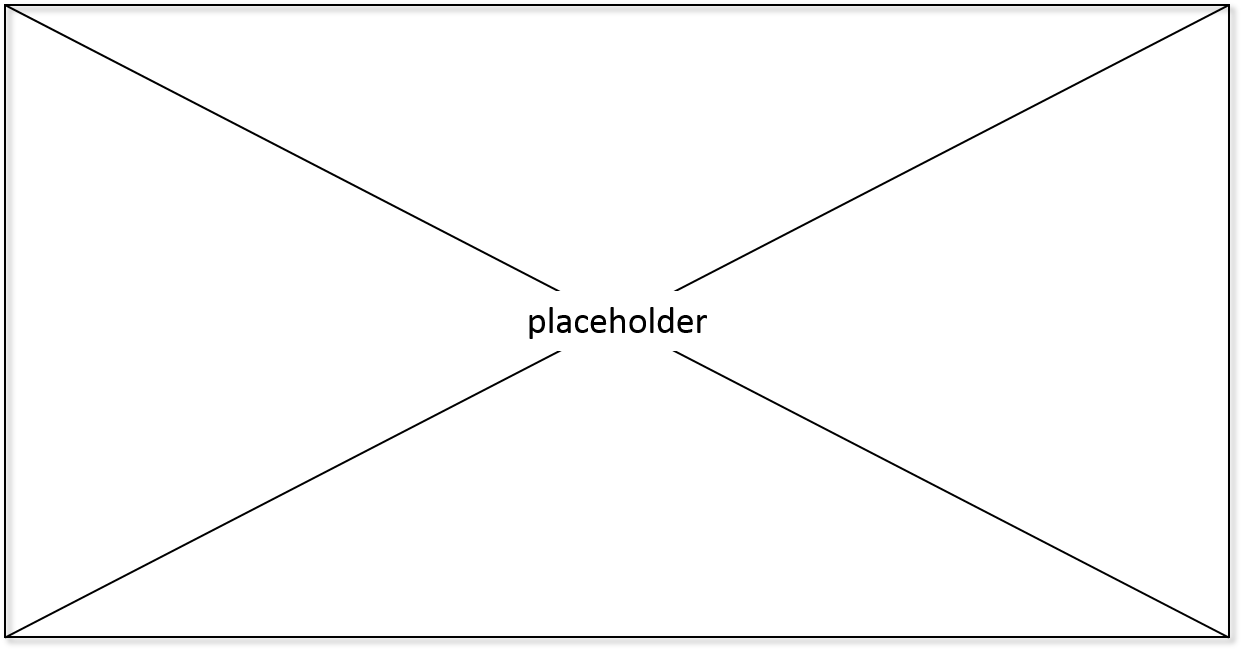
\includegraphics[trim= 0 0 0 0, clip,width=2cm]{placeholder.png}}
\fancyfoot[L]{}
\fancyfoot[C]{}
\fancyfoot[R]{\thepage}
%lines on header and footer
\renewcommand{\headrulewidth}{0.5pt}
\renewcommand{\footrulewidth}{0.5pt}

% Style of cite
\usepackage[style=authoryear,backend=biber,sorting=nyt]{biblatex}
%Add your bib file here
%\addbibresource{literature.bib}